\documentclass[letter, 10pt]{article}
\usepackage{fullpage}
\usepackage[margin=0.5in]{geometry}
\usepackage{graphicx}
\usepackage{wrapfig}
\usepackage{caption}
\usepackage{subcaption}
\usepackage{listings}
\usepackage{hyperref}
\usepackage{amsmath}
\usepackage{float}

\pagenumbering{gobble}

\begin{document}
\noindent
\large \textbf{Rahul Ghosh} \hfill \textbf{Assignment\#4}\\
\normalsize Student ID: 5476965 \hfill CSci 5561\\

\section*{\centering CONVOLUTIONAL NEURAL NETWORK}

\subsection*{Methods}
\subsubsection*{Single-layer Linear Perceptron}
A single-layer linear perceptron is used as a model to classify the images. Euclidean distance between the prediction and true label is used as the objective function and Stochastic gradient descent is used as an optimizer to train the model.\\
\underline{Optimizer Parameters}: learning\_rate = 0.01\quad decay\_rate = 1\\
The results are shown in Figure 1.

\subsubsection*{Single-layer Perceptron}
A single-layer perceptron is used as a model to classify the images. Cross entropy loss between prediction and true label is used as the objective function and Stochastic gradient descent is used as an optimizer to train the model.\\
\underline{Optimizer Parameters}: learning\_rate = 0.6\quad decay\_rate = 0.9\\
The results are shown in Figure 2.

\subsubsection*{Multi-layer Perceptron}
A multi-layer perceptron with 1 hidden layer of 30 units is used as a model to classify the images. Cross entropy loss between prediction and true label is used as the objective function and Stochastic gradient descent is used as an optimizer to train the model.\\
\underline{Optimizer Parameters}: learning\_rate = 0.6\quad decay\_rate = 0.99\\
The results are shown in Figure 3.

\subsubsection*{Convolutional Neural Network}
A convolutional neural network with 1 hidden layer of 30 units is used. Cross entropy loss between prediction and true label is used as the objective function and Stochastic gradient descent is used as an optimizer to train the model.\\
\underline{Optimizer Parameters}: learning\_rate = 0.6\quad decay\_rate = 0.99\\
The results are shown in Figure 4.

\subsection*{Results}
\begin{figure}[H]
    \minipage{0.33\textwidth}
        \centering
        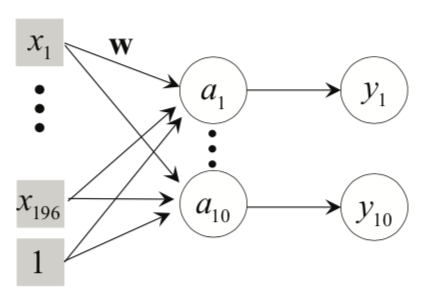
\includegraphics[width=\textwidth]{HW4/RESULT/SLP_linear.png}
        \subcaption{Single-layer Linear Perceptron}
    \endminipage\hfill
    \minipage{0.33\textwidth}
        \centering
        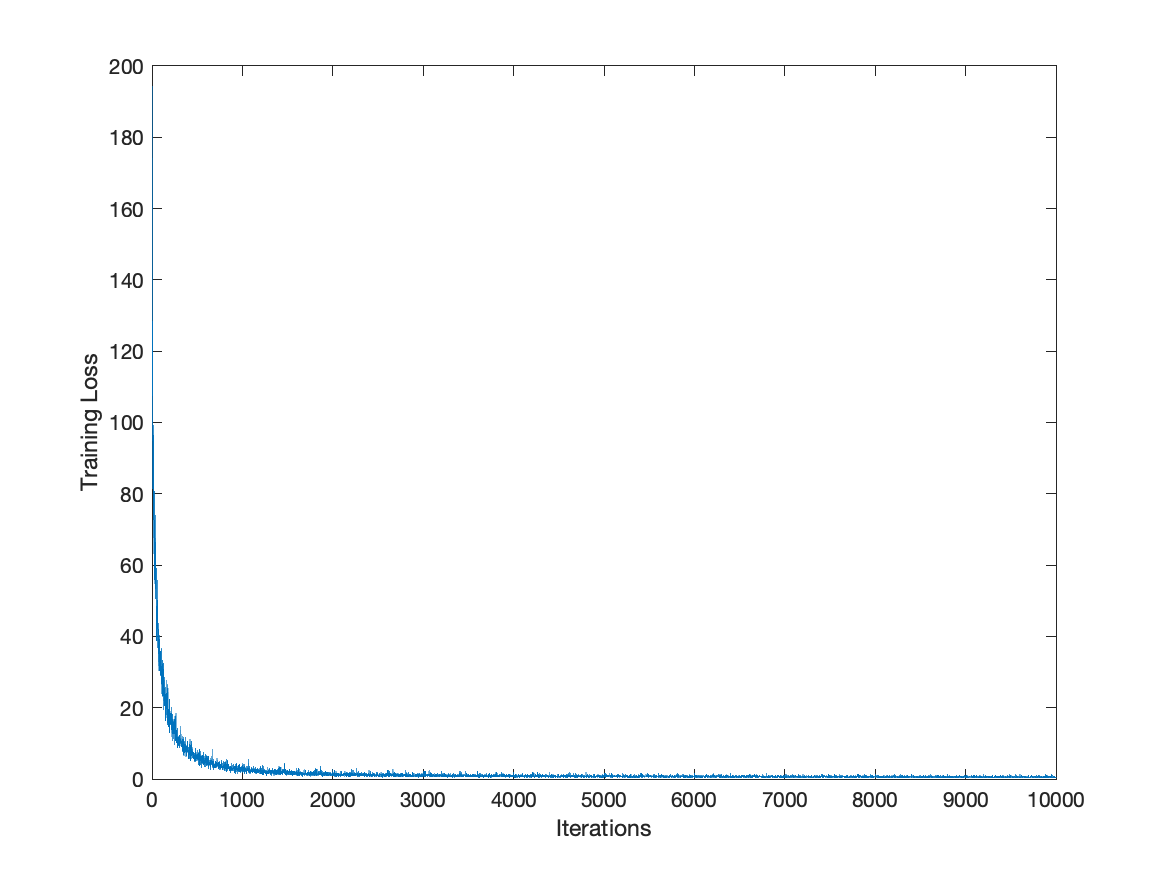
\includegraphics[width=1.1\textwidth]{HW4/RESULT/SLP_linear_loss.png}
        \subcaption{Training Loss}
    \endminipage\hfill
    \minipage{0.33\textwidth}
        \centering
        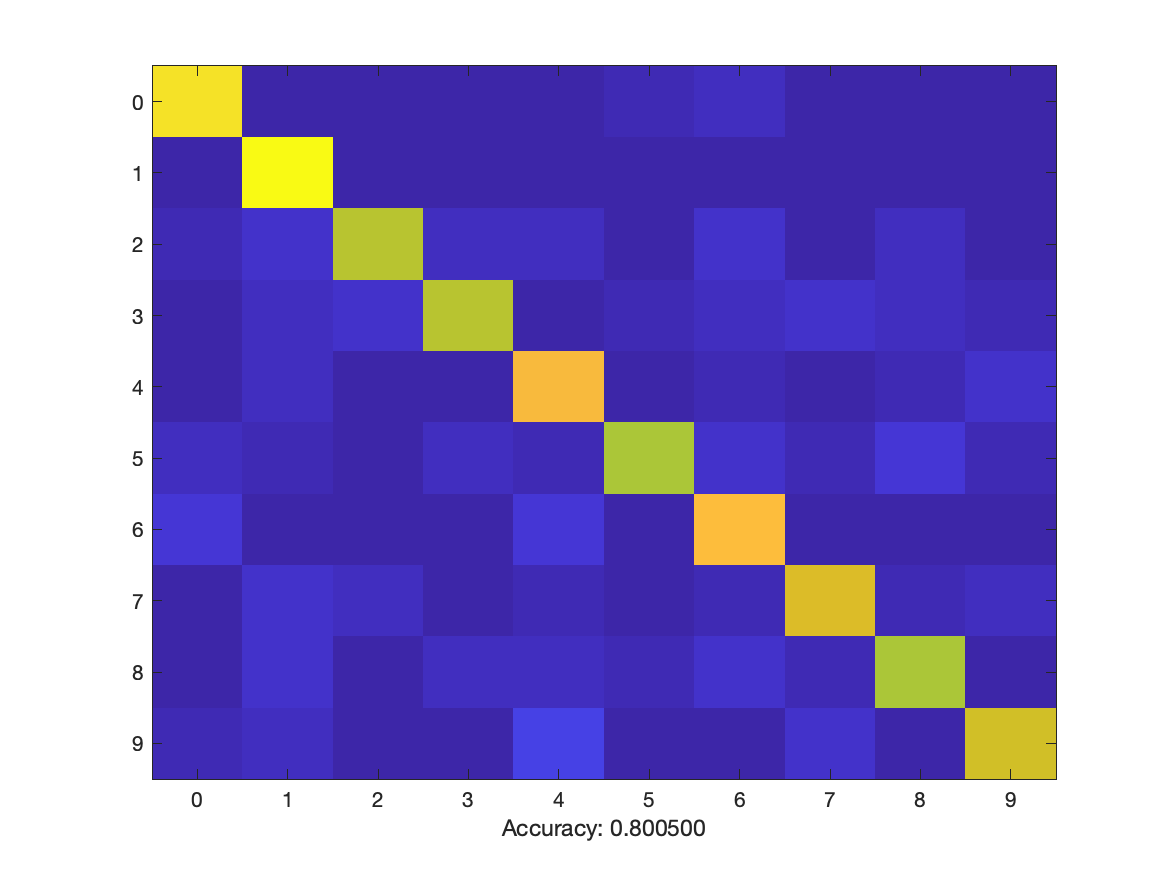
\includegraphics[width=1.1\textwidth]{HW4/RESULT/SLPLINEAR_CONFUSION.png}
        \subcaption{Tiny Image}
    \endminipage\hfill
    \caption{Single-layer Linear Perceptron}
\end{figure}

\begin{figure}[H]
    \minipage{0.33\textwidth}
        \centering
        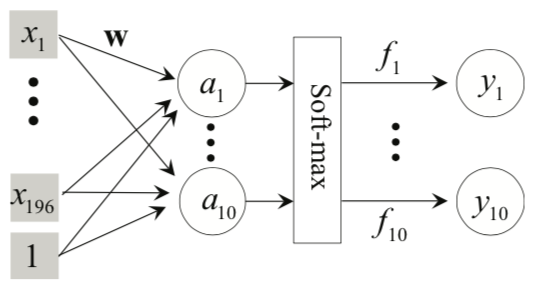
\includegraphics[width=\textwidth]{HW4/RESULT/SLP.png}
        \subcaption{Single-layer Linear Perceptron}
    \endminipage\hfill
    \minipage{0.33\textwidth}
        \centering
        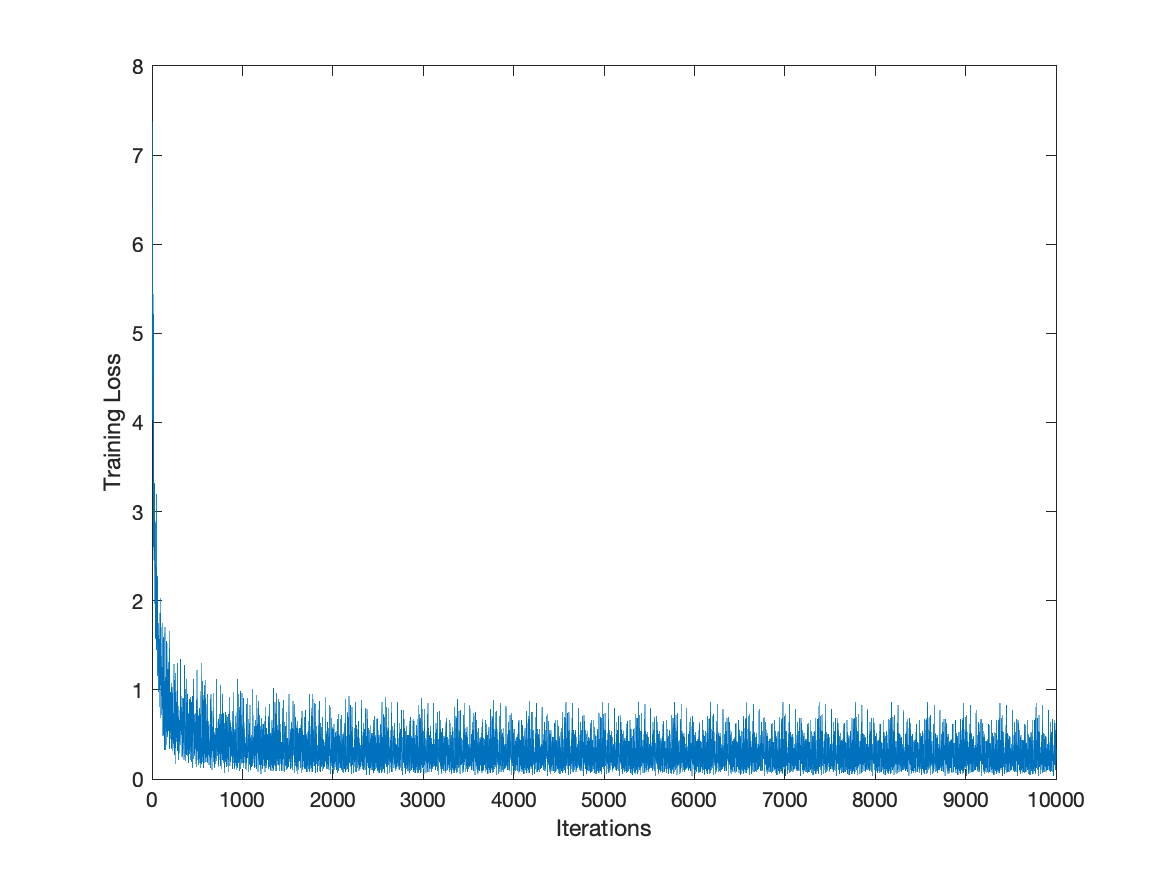
\includegraphics[width=1.1\textwidth]{HW4/RESULT/SLP_loss.png}
        \subcaption{Training Loss}
    \endminipage\hfill
    \minipage{0.33\textwidth}
        \centering
        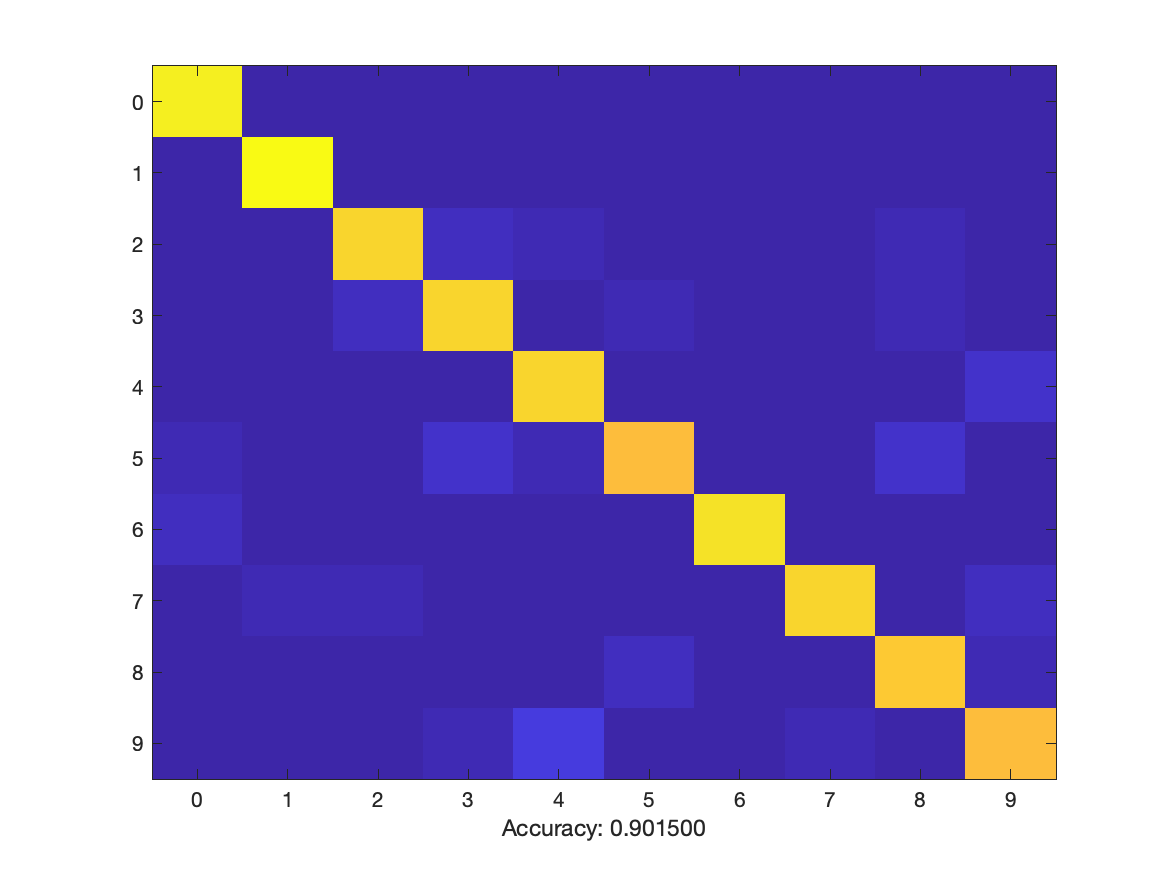
\includegraphics[width=1.1\textwidth]{HW4/RESULT/SLP_CONFUSION.png}
        \subcaption{Tiny Image}
    \endminipage\hfill
    \caption{Single-layer Perceptron}
\end{figure}

\begin{figure}[H]
    \minipage{0.33\textwidth}
        \centering
        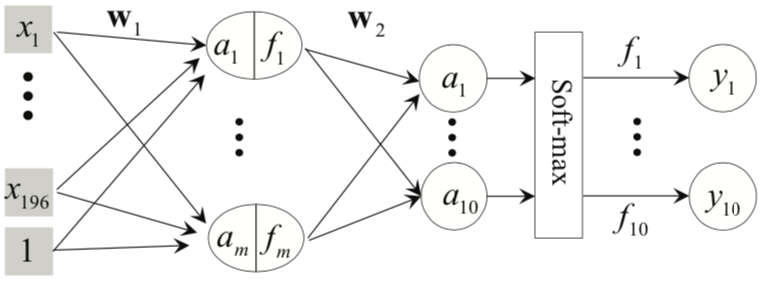
\includegraphics[width=\textwidth]{HW4/RESULT/MLP.png}
        \subcaption{Single-layer Linear Perceptron}
    \endminipage\hfill
    \minipage{0.33\textwidth}
        \centering
        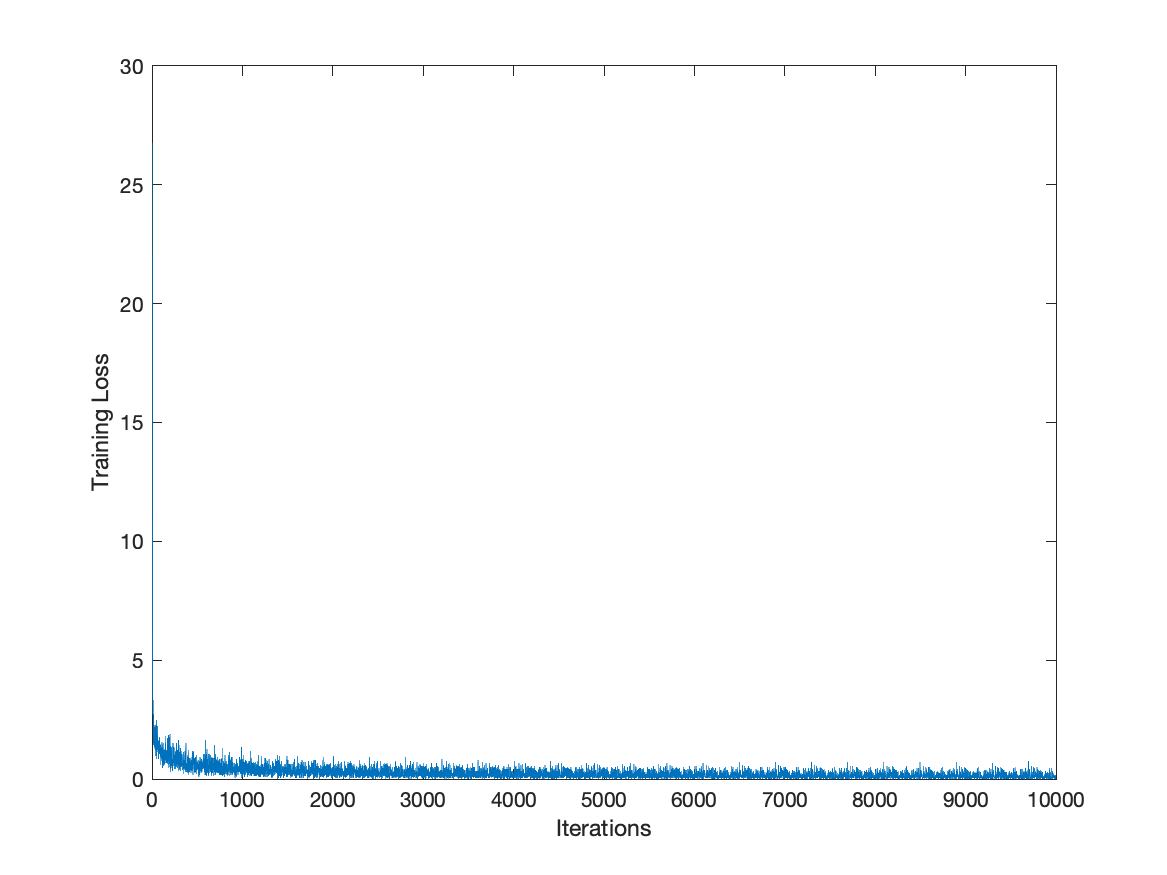
\includegraphics[width=1.1\textwidth]{HW4/RESULT/MLP_loss.png}
        \subcaption{Training Loss}
    \endminipage\hfill
    \minipage{0.33\textwidth}
        \centering
        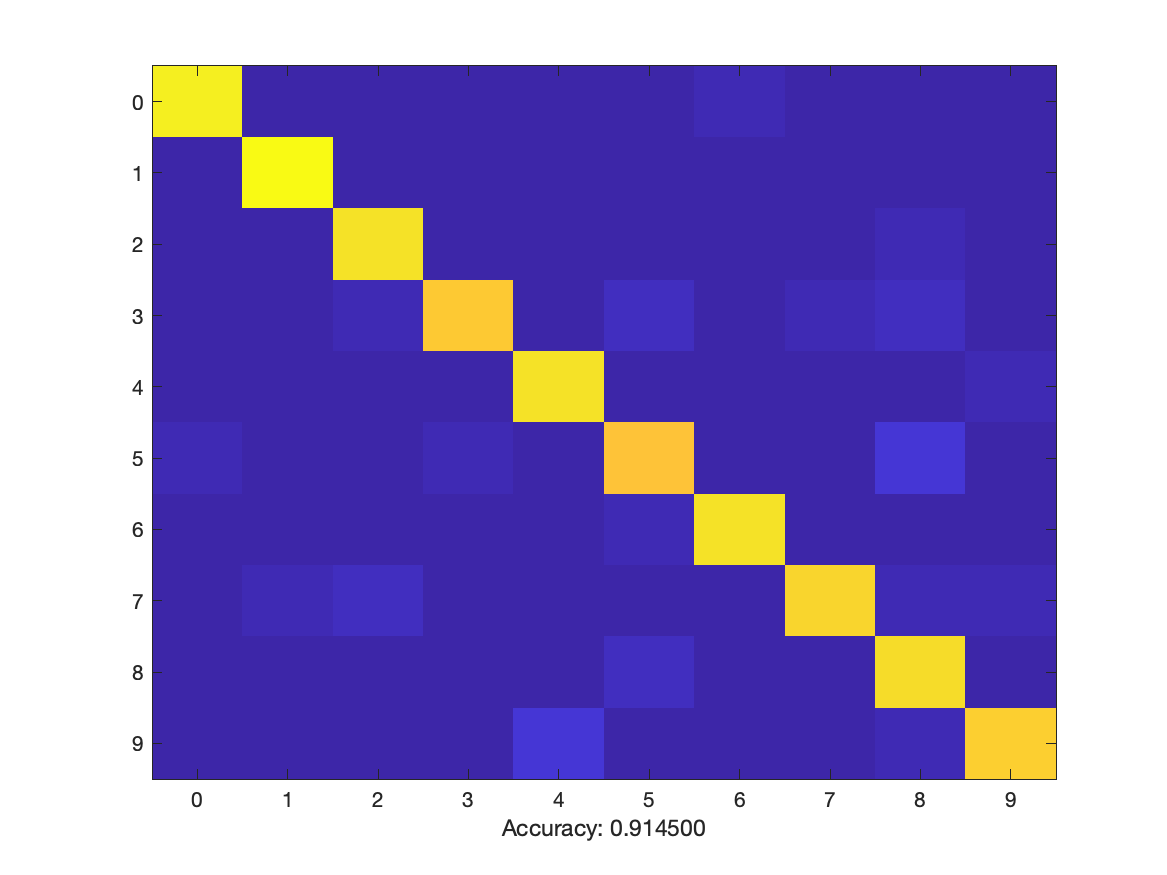
\includegraphics[width=1.1\textwidth]{HW4/RESULT/MLP_CONFUSION.png}
        \subcaption{Tiny Image}
    \endminipage\hfill
    \caption{Multi-layer Perceptron}
\end{figure}

\begin{figure}[H]
    \minipage{0.33\textwidth}
        \centering
        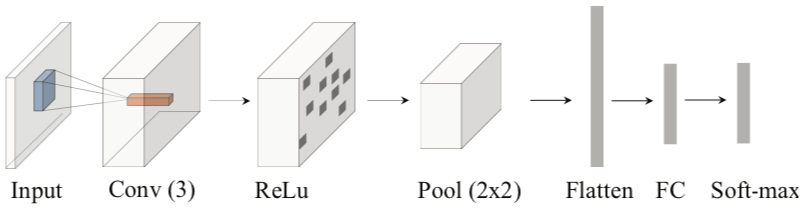
\includegraphics[width=\textwidth]{HW4/RESULT/CNN.png}
        \subcaption{Single-layer Linear Perceptron}
    \endminipage\hfill
    \minipage{0.33\textwidth}
        \centering
        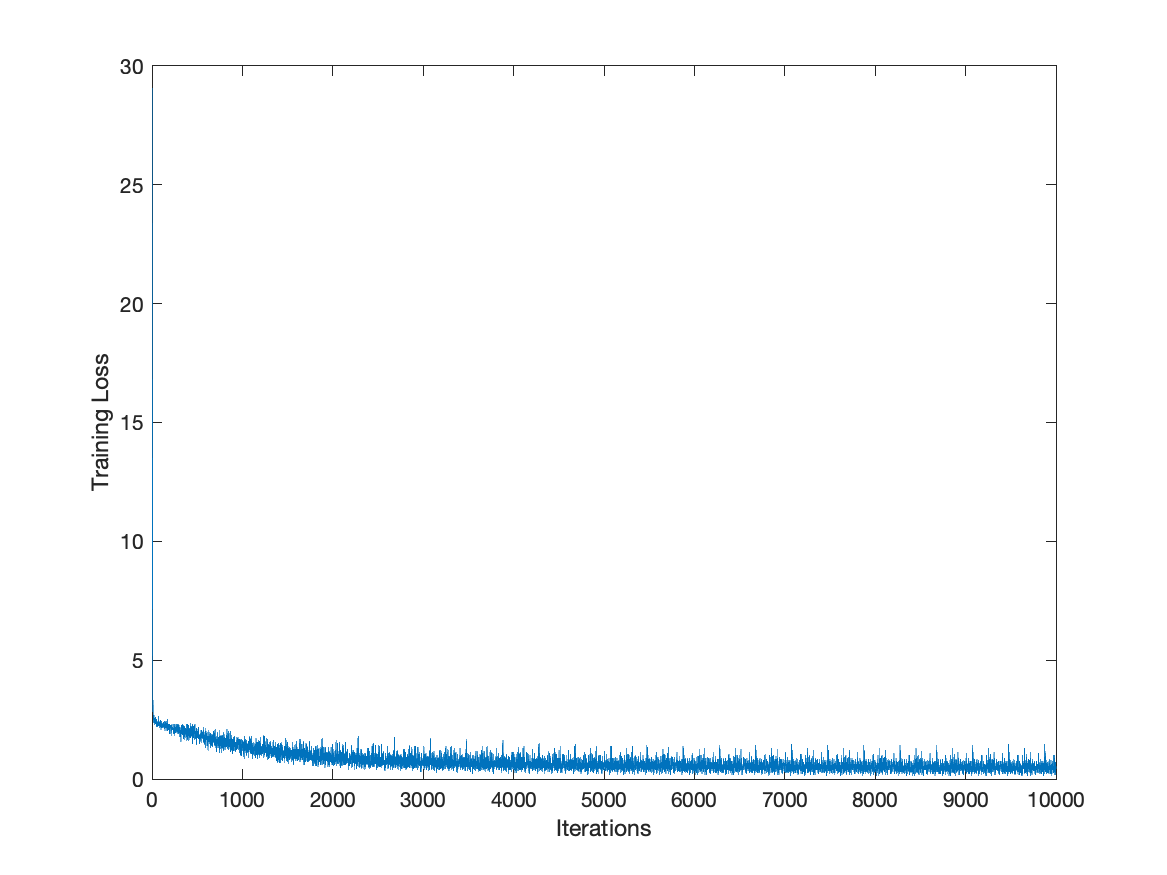
\includegraphics[width=1.1\textwidth]{HW4/RESULT/CNN_loss.png}
        \subcaption{Training Loss}
    \endminipage\hfill
    \minipage{0.33\textwidth}
        \centering
        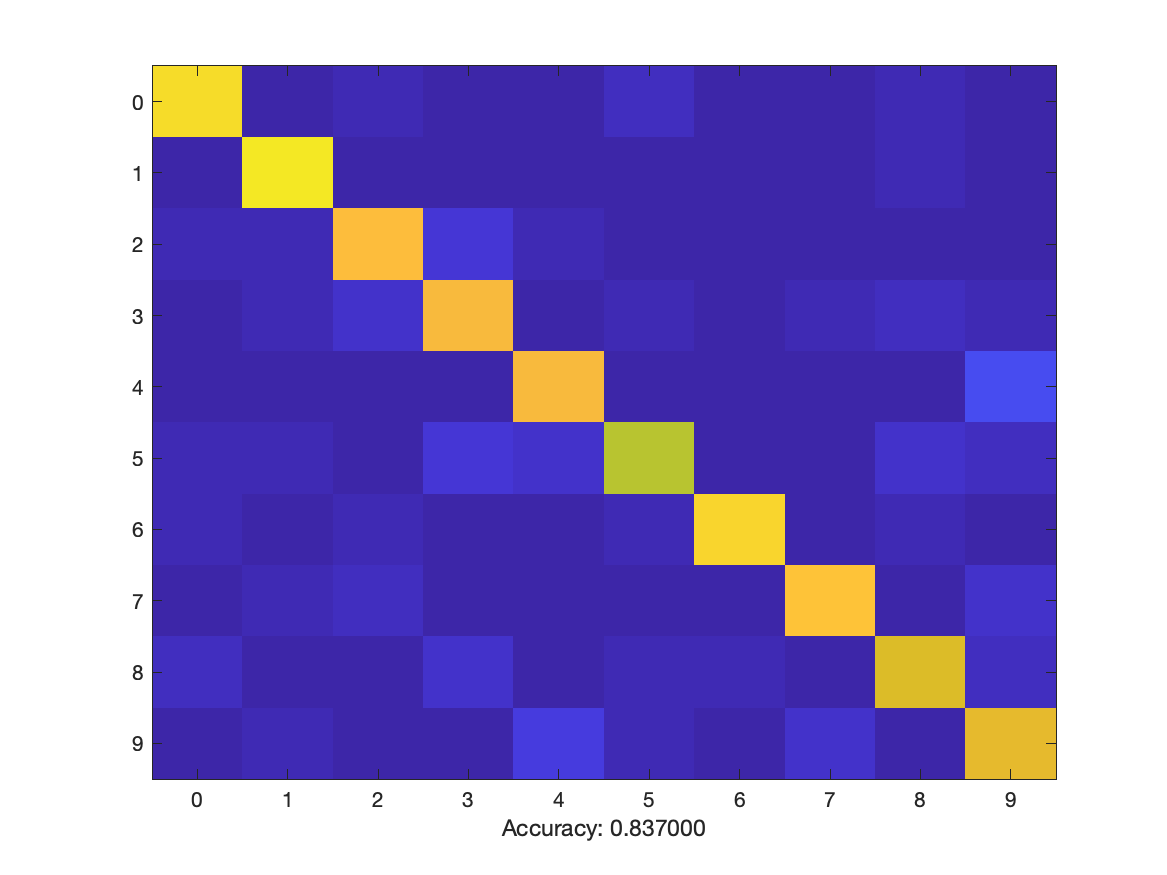
\includegraphics[width=1.1\textwidth]{HW4/RESULT/CNN_CONFUSION.png}
        \subcaption{Tiny Image}
    \endminipage\hfill
    \caption{Convolutional Neural Network}
\end{figure}
\end{document}